\chapter{Language}
\label{chap:language}

We have seen that people easily learn associations, and can use them for prediction about the future. People integrate information from the recent past to make predictions \notet. We also know that human memory systems are optimized for storing $7 \pm 3$ items, and that chunking is one of the main tools used to construct these items. All this suggests that our ability to use learned associations, keep track of the recent past, and make predictions would be fundamental for \textbf{language comprehension} as well.

\osst{Note: some researchers think people do not make predictions on the next word. But once the word is received, then the fit of the new word given the previous context is computed. If the fit is low, then the surprise is high. There is huge debate whether people make predictions.}

In the following we try to answer the two main questions underlying modern and less modern theories of language:
\begin{itemize}
    \item do we store language associations?
    \item if so, how do we use them for comprehension?
\end{itemize}

\section{Language comprehension and integration}
There are different theories on how humans learn what is a grammatically valid sentence in a language:
\begin{itemize}
    \item From experience, we \textbf{memorize structures}: which can be words or types of phrases that go together. In this case a fundamental role is played by memory, to store statistics;
    \item We learn \textbf{abstract rules} that specify constraints on grammaticality;
    \item We acquire \textbf{statistical knowledge} on co-occurrence of language entities. This approach considers memorization and abstract rules to be wrong, as we do not need to acquire precise memorization nor rules.
\end{itemize}
These three approaches on the human ability to understand Language have been ``fighting" for a long time, however they are not necessarily dichotomous.

\subsection{Memorization of structures (Behavioral psychology)}
This approach took off with the advent of \textbf{behavioral psychology}.
Behavioral psychology research applied S-R (Stimulus-Response) models for language: each word is thought of being a stimulus for the next, building up an overall structure out of local associative relations.
In language comprehension, the learned sequences of \textbf{adjacent elements} are internally represented as automatically characterizing a sentence as it is encountered. In other words, we \textbf{parse the sentence as a set of local associations}, and then we see if the occurrences have been already encountered (i.e., are stored in the memory). This allows us to determine if it is grammatically correct. We would say (today) that on behaviorism, knowledge of language is 
knowing which words/elements are followed by other words, which is a very simple idea, but assumes we have a huge amount of memory.
Moreover, it does not explain how \textit{meaning} is made, but it explains how people produce valid sentences to communicate an idea: they know which words/elements can come after others.
We use the term ``\textbf{element}" because instead of learning associations between words, people maybe have the ability to learn associations between part-of-speech elements.

\subsubsection{Elements in S-R approaches to language}
S-R approaches claim we learn which words come after each other, e.g.:\\
$Horse \rightarrow races$ (relation between specific lexical items)\\
But they also allow for some abstraction, which enable ``slots". E.g. patterns such as:
\begin{enumerate}
    \item $\text{The} \rightarrow X \rightarrow Y\text{-es}$ (relation between definite article, noun [singular], verb [singular]
    \item $\text{The} \rightarrow X\text{-es}\rightarrow Y\_$ (relation between definite article, plural noun, plural verb)
\end{enumerate}
This is more compact than storing single words' associations. However, this compression requires people to have part-of-speech categories.

\subsubsection{Abstract elements in sentence level}

\begin{wrapfigure}[8]{r}{0pt}
  \centering
  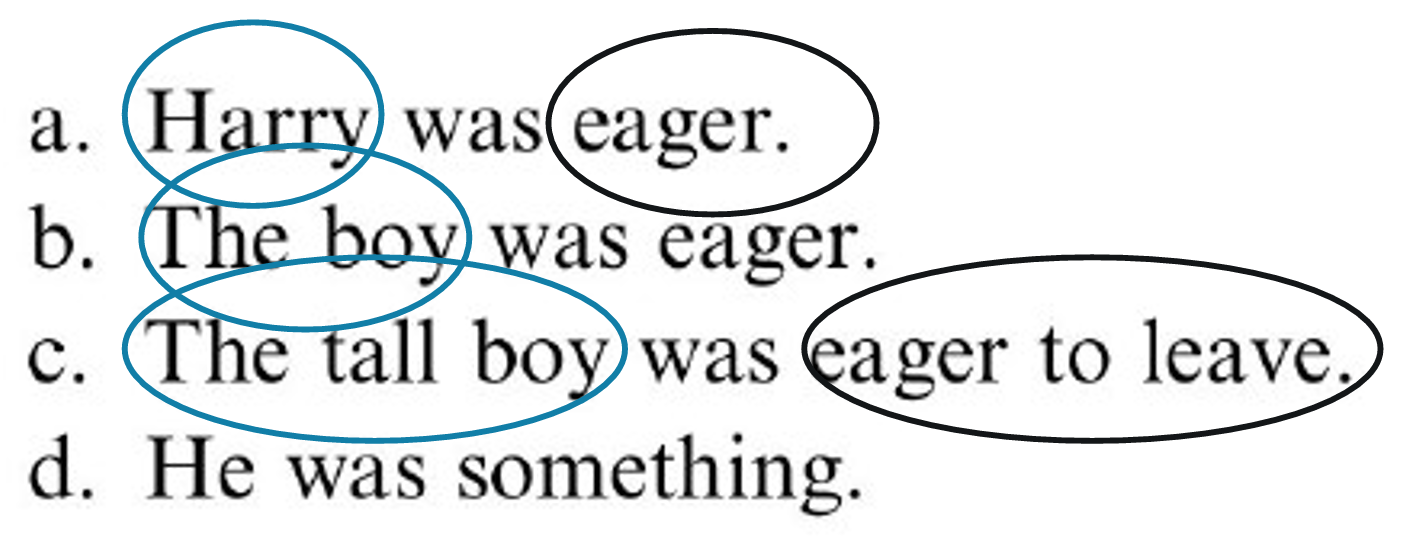
\includegraphics[width=0.3\textwidth]{images/elements.png}
  \caption{}
  \label{fig:elements}
\end{wrapfigure}
If people can memorize such paradigm (phrase structure as an element). Then maybe they can also learn what phrase structure can substitute in longer phrases.

This is what Behaviorists believed, accepting some level of abstraction. They attempted to describe different types of phrases. They accepted that longer phrases seemed to resolve into combinations of shorter ones, which in turn could resolve into single words. In other words, longer phrases can be shortened recursively, until a minimal sentence is reached, to know if they are grammatically correct or not (Fig.~\ref{fig:elements}).
The original S-R approach is no more easily visible here.
Moreover, they did not really have a theory for storing word meaning.

\subsubsection{Meaning in S-R approaches to language}
Behaviorists did not develop theories about mental phenomenon (e.g. theories of conceptual representation). They had several parallel ideas.
The first one is the {Substitution view}: words (``signs") substituted for the objects in the world. Objects in the world produce a real reaction, and the sign produces a similar reaction.  Therefore, the meaning of a word is the response it produces in a person (quite neuro-scientific idea \notet). The substitution view has a problem, it does not work for words with meanings we never experienced. So an alternative was offered by Osgood (1952), the \textbf{Disposition view}: language produces a tendency (\textit{disposition}) towards certain behaviors. ``\textit{The meaning of a linguistic expression is therefore disposition towards response sequence}".

\osst{\colorbox{yellow!20}{Digression:} There are neurons that fire in the same way during production (e.g. moving the hand) and perception (seeing someone moving the hand). This means there is some sort of common categorization.}

\subsection{Abstract rules (Chmosky grammar)}
Chomsky (1959) challenged S-R learning and behaviorism, identifying multiple weaknesses. His two main arguments were:
\begin{itemize}
    \item inability to explain comprehension of sentences not heard previously,
    \item inability to handle hierarchical structure and long-distance dependencies.
\end{itemize}

There is evidence of humans understanding of language as constrained by a grammar with abstract rules.
In an experimental setup, when people hear single words distorted by noise, they correctly recognize 25\% of the words. Assuming words are mapped independently, we would assume an accuracy of 6.25\% when 2 words are put together, but we get 50\%. This means we have a grammatical knowledge with constraints that are used when hearing: ``acoustic representation" is not mapped independently per word.\\

This evidence opened the door to the question of how does knowledge of sentences impact comprehension, where top-down explanation have been battling bottom-up ones for over 60 years.
Things are clearer in sentences because the constraints are not from rote memory, but from more abstract systems of rules: so adults develop representations that cannot be directly derived from prior experience.

\subsubsection{Transformational grammar}
For Chomsky (1957) a sentence is what the grammar describes it as a sentence.
His grammar is generative: it describes the sentence structures of a language as a natural and creative part of human knowledge.
Grammar constitutes a theory of the speaker’s underlying linguistic 
knowledge. It is not concerned with the (noisy) actual behavior or its importance for the study of language.\\

\begin{wrapfigure}[8]{r}{0pt}
  \centering
  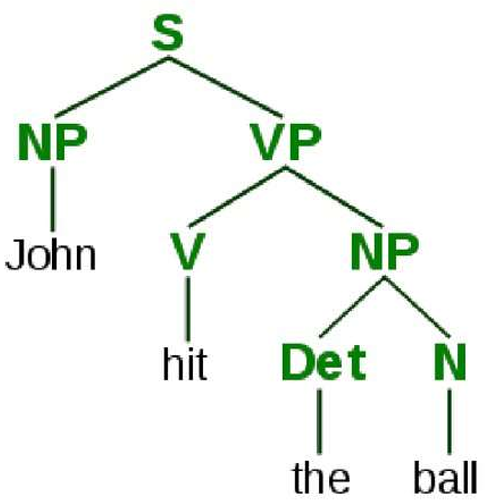
\includegraphics[width=0.2\textwidth]{images/tree.png}
  \caption{}
  \label{fig:tree}
\end{wrapfigure}

\textbf{\textit{Sentence meaning} is captured by its structure}. Structures ``licensed" by the grammar of a language are those that can be produced by the language's grammar (\textbf{\textit{rewrite rules}}). The importance of describing sentences this way is that similar sentences can have very different grammatical structures (or vice versa, e.g. \textit{John is easy to please} and \textit{John is eager to please} are sentences with very similar surface structures but very different meaning).

Sentences are represented as trees, with the \textbf{Chomsky hierarchy} (an example is provided in Fig.~\ref{fig:tree}). As sentence meaning is related to its structure, it is possible to disambiguate ambiguous strings of words.

\subsubsection{Derivational theory of psychological complexity}
These ideas can be used to build a psychological theory: the \textbf{derivational theory of complexity} (DTC), the first theory that tried to account for difficulty of sentence comprehension. It is innovative in that it identified an objective metric on which complexity can vary, and examined correlations between value of this metric and human behavior. The metric was the \textbf{number of transformations needed to transform a kernel sentence to a given sentence} (very similar to the substitutions seen in the behavioralist approach). The entire sentence was taken as a unit, and a set of pre-set rules (a grammar) was used to see if the given sentence can be derived from the kernel sentence. \textbf{No incremental parsing} was used.

\begin{figure}[!ht]
    \centering
    \captionsetup{width=.8\linewidth}
    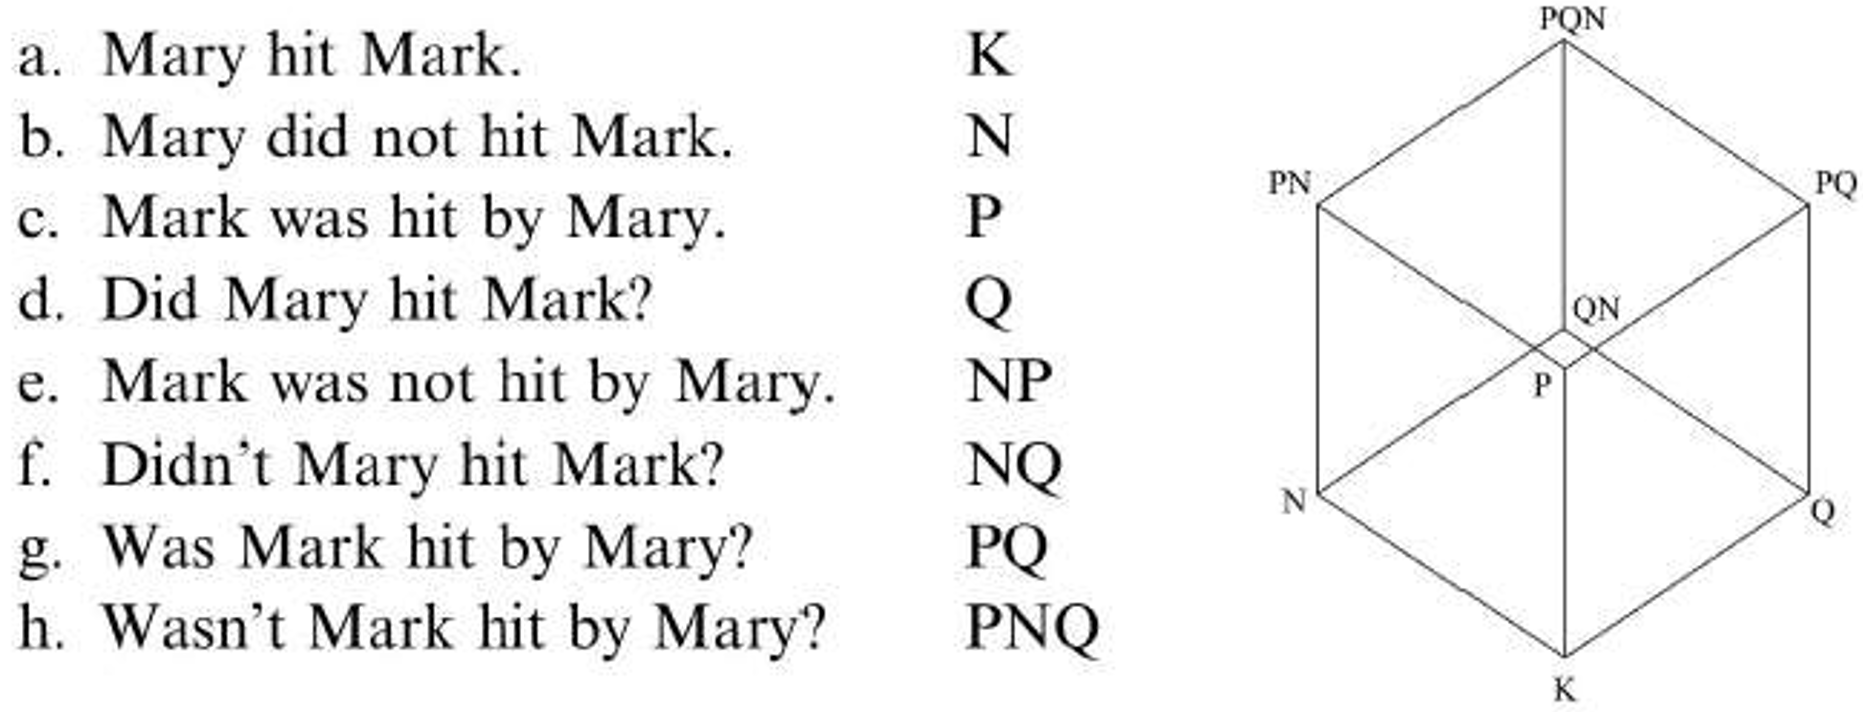
\includegraphics[width=0.5\linewidth]{images/dtc.png}
    \caption*{DTC: the complexity of a sentence is its distance from the kernel sentence (i.e., how many transformations are needed).}
    \label{fig:dtc}
\end{figure}

DCT enjoyed some early success, particularly when using sentence-picture verification studies, as the verification time can be predicted by the complexity (e.g. the verification time of ``\textit{The boy smelled the flower}" is lower than that of ``\textit{The flower was smelled by the boy}").
DTC was eventually abandoned because of criticisms to the method (construct validity) and findings suggesting these effects have to do with how the photo might be encoded into language. The other problem with this theory is that there is no incremental parsing, despite people do parse sentences (and predict what comes next). This theory completely ignores this aspect.

\subsubsection{Parsing-based accounts}
Parsing is an incremental process by which we try to assign a structure to what we have read/heard. In some cases we experience local ambiguity that slows down our comprehension. Such ambiguity is, in many cases, local and is disambiguated by later content. Parsing-based accounts try to explain \textbf{why some tentative interpretations are preferred} and why some sentences are more difficult.\\

We have evidence that humans try to parse sentences: there are particular type of structures, e.g. ``The horse raced past the barn fell". People parse this sentence in a preferred way until ``barn", and at that point they expect the end of the sentence, but encounter ``fell" instead, which makes the whole past parsing wrong. This proves humans do parsing in real time, but also that they make predictions during language comprehension (anticipatory predictions).\\

We also have evidence for anticipation (people make predictions while they understand language) thanks to the \textbf{visual world paradigm} experiment. Participants hear utterances while looking at a visual display of target word along with competitors and distracters. The task assigned to the participants is to look while listening. In Fig. \ref{fig:vwp_1} are the results; the slight advantage of ``\textit{cake}" even before the noun offset is maybe because the boy is looking at it. From these results we cannot rule out the possibility that people actually make predictions.

\begin{figure}[!ht]
    \centering
    \captionsetup{width=.8\linewidth}
    \begin{subfigure}{.42\textwidth}
        \centering
        \captionsetup{width=.8\linewidth}
        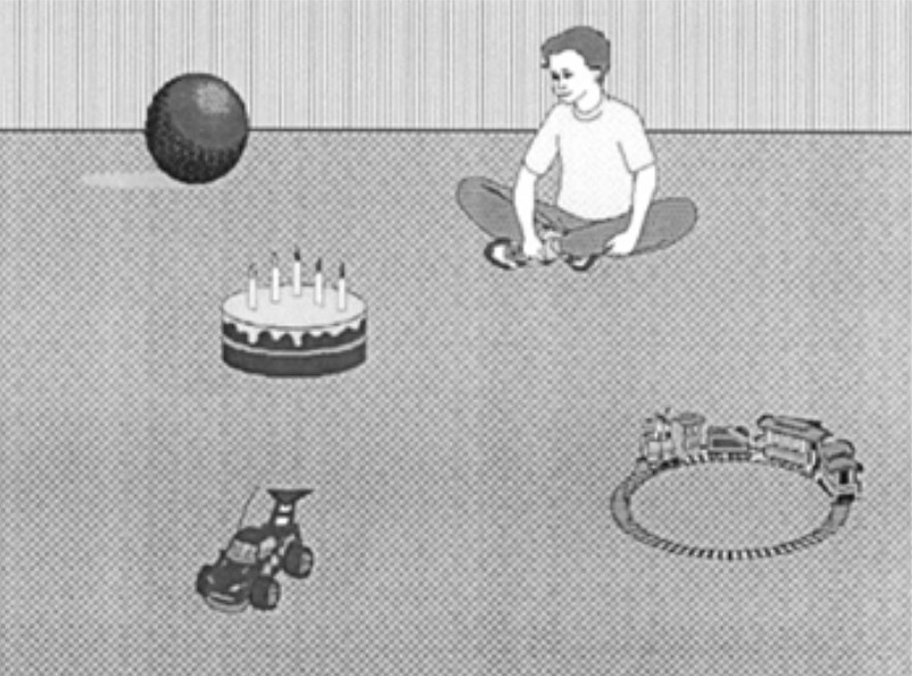
\includegraphics[width=.9\linewidth]{images/vwp.png}
        \caption{}
        \label{fig:vwp}
    \end{subfigure}
    \begin{subfigure}{.56\textwidth}
        \centering
        \captionsetup{width=.8\linewidth}
        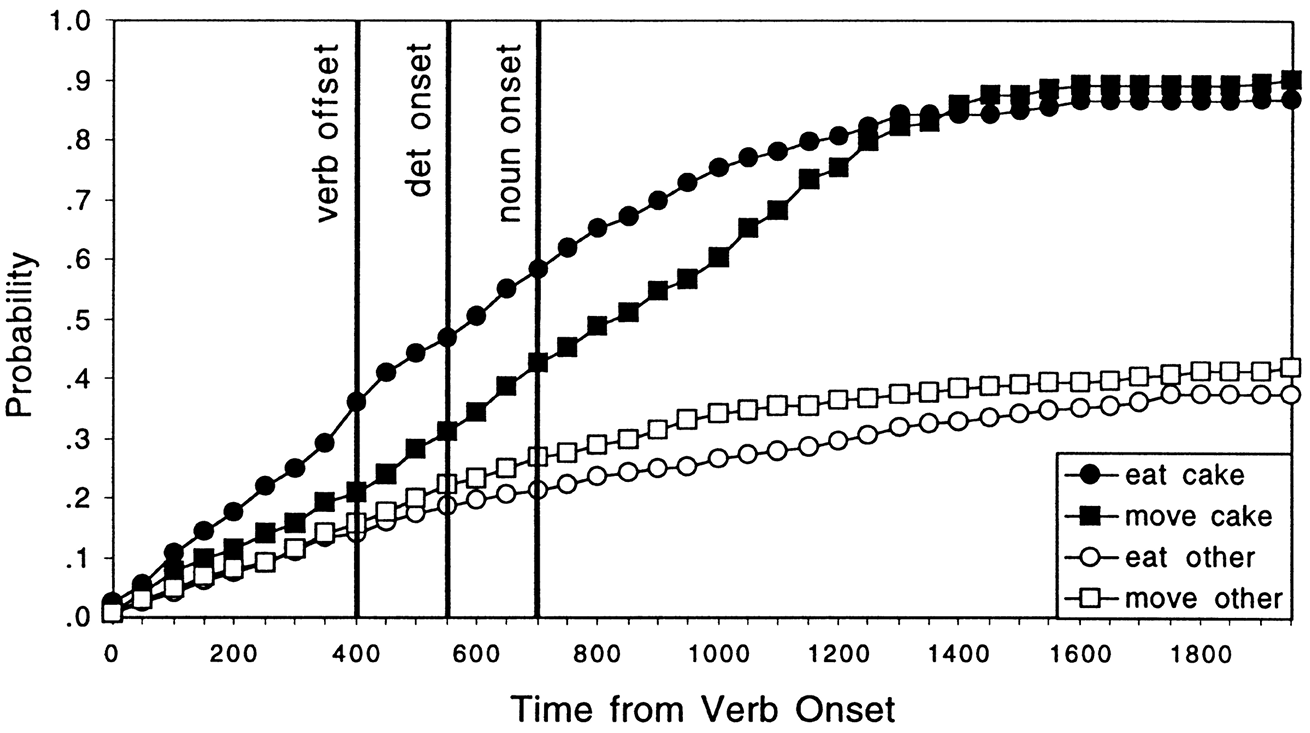
\includegraphics[width=.9\linewidth]{images/vwp_2.png}
        \caption{}
        \label{fig:vwp_2}
    \end{subfigure}
    \caption{Visual World Paradigm by Altmann and Kamide (1999). \textbf{(a)} Task: Look at the picture while hearing ``the boy will move the cake". \textbf{(b)} The cumulative probability of fixating the target object (cake) or a distractor (other) as a function of condition (``eat" vs.~``move). Note: the verb offset, determiner onset, and noun onset, averaged across trials, are shown aligned to the 50 ms bin within which they fell.}
    \label{fig:vwp_1}
\end{figure}

\section[Support for structure-pruning/surprisal]{Support for structure-pruning/surprisal\\ \textit{Insensitivity of the Human Sentence-Processing System to Hierarchical Structure}\\
\mandatory{frank}}
AI researchers started seeing how grammars and rules are not necessary for learning something: the exposure to data can make the models learn the underlying probability distributions. \cite{frank} assume that comprehension is based on structure building; they test the idea by comparing 3 models of language:

\begin{wrapfigure}[13]{r}{0pt}
  \centering
  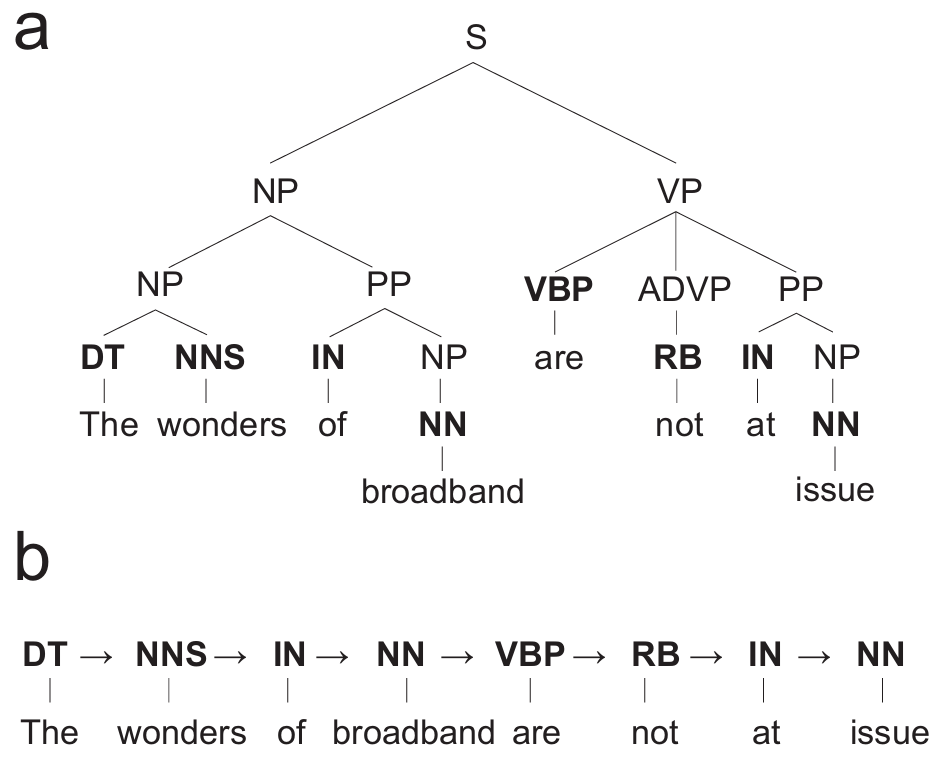
\includegraphics[width=0.4\textwidth]{images/frank.png}
  \caption{Example of \textbf{(a)} hierarchical phrase structure and \textbf{(b)} sequential structure for a sentence.}
  \label{fig:frank}
\end{wrapfigure}
\begin{itemize}
    \item Probabilistic PSG (Phrase-Structure Grammar)
    \item Markov process (N-gram)
    \item Echo state network (ESN, similar to vanilla RNN)
\end{itemize}
They define the \textbf{model quality} as the \textbf{accuracy of predicting human behavior}. PSG models use hierarchical structures (see Fig. \ref{fig:frank}a), whereas Markov models and ESNs estimate probabilities that depend solely on the sentences' sequential structure (as shown in Fig. \ref{fig:frank}b).\\

As training set, they use the ``Wall Street Journal" corpus (49k sentences). This corpus has a syntactic-structure tree annotation for each sentences, which is ideal for training Probabilistic PSG.
For Markov models and ESNs, they replaced each word with its Part-of-Speech category, so that the models learn to predict POS instead of specific word. This improves accuracy for small 
datasets. Also, this way there is no need for an algorithm to learn to predict highly specific semantics, as syntactic POS is the target for prediction.

\subsection{Probabilistic PSGs}
They experiment with different types of PSG:
\begin{itemize}
    \item a classic which just considers what continuations can follow each phrase (memory-less);
\end{itemize}

\begin{itemize}
    \item $n$\textsuperscript{th} order versions, which consider which continuations can follow combinations of phrases.
\end{itemize}

\begin{wrapfigure}[8]{r}{0pt}
  \centering
  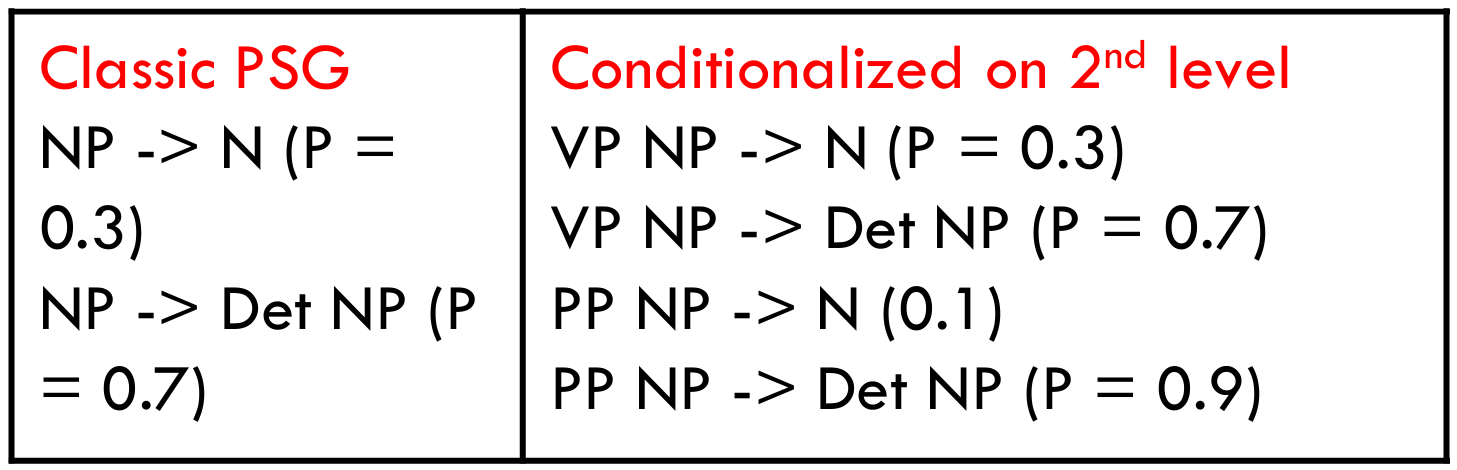
\includegraphics[width=0.34\textwidth]{images/psg.png}
  \caption{}
  \label{fig:psg}
\end{wrapfigure}

In a standard probabilistic context-free grammar, the probability that a parent node will produce a particular set of children is conditional only on the parent node, but it is well known that parsing accuracy can be improved by taking the grandparent node (e.g. in Fig. \ref{fig:frank}a, VP, or verb phrase, is the grandparent of the rightmost IN and NP) into account. Likewise, a rule's probability can be made conditional on information from even higher up in the parse tree. This motivates the $n$\textsuperscript{th} order versions. A comparison is provided in Fig. \ref{fig:psg}.\\

In addition, in an effort of capturing as much structural knowledge as possible, they induced four more PSGs, in which conditioning information was taken not only from ancestor nodes (e.g. grandparent nodes) but also from the ancestors' left siblings (e.g. in Fig. \ref{fig:frank}a, the left sibling of VP is NP), again varying the maximum number of levels up in the tree from one to four. In this manner, they obtained highly structurally sensitive syntactic models. Fig. \ref{fig:psg_2} highlights the differences.

\begin{figure}[!ht]
    \centering
    \captionsetup{width=.8\linewidth}
    \begin{subfigure}{.32\textwidth}
        \centering
        \captionsetup{width=.8\linewidth}
        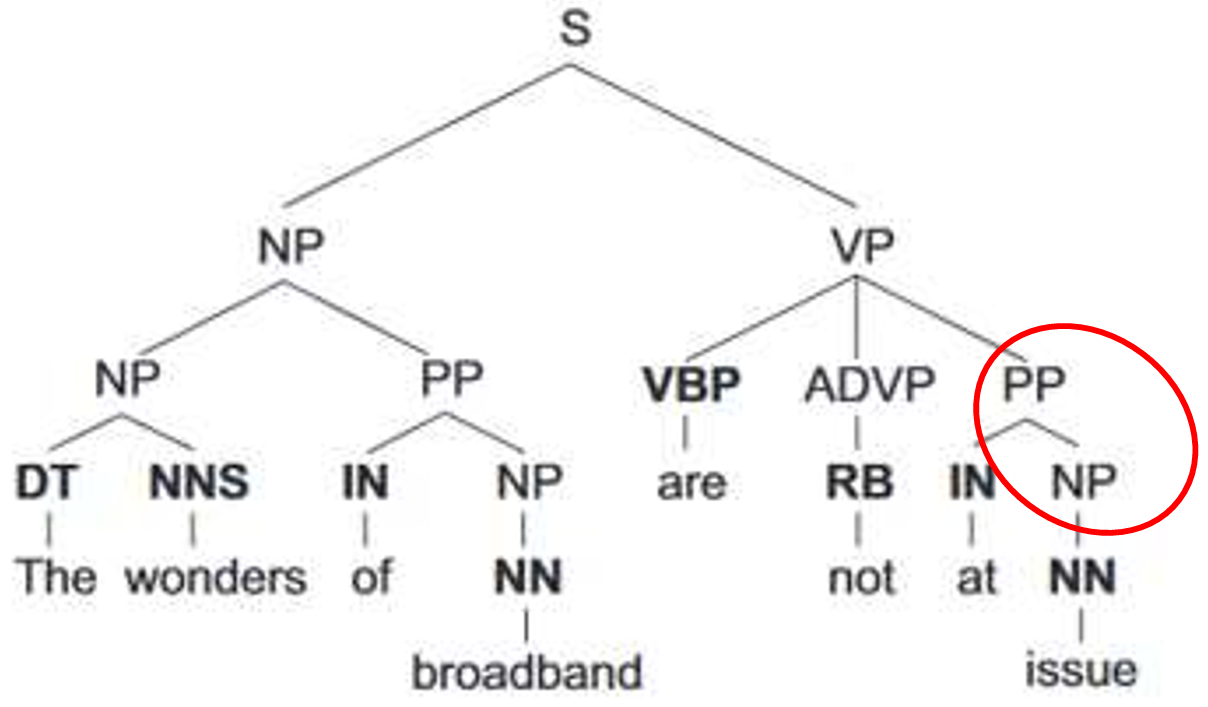
\includegraphics[width=.9\linewidth]{images/psg_1.png}
        \caption*{Regular probabilities.}
    \end{subfigure}
    \begin{subfigure}{.32\textwidth}
        \centering
        \captionsetup{width=.8\linewidth}
        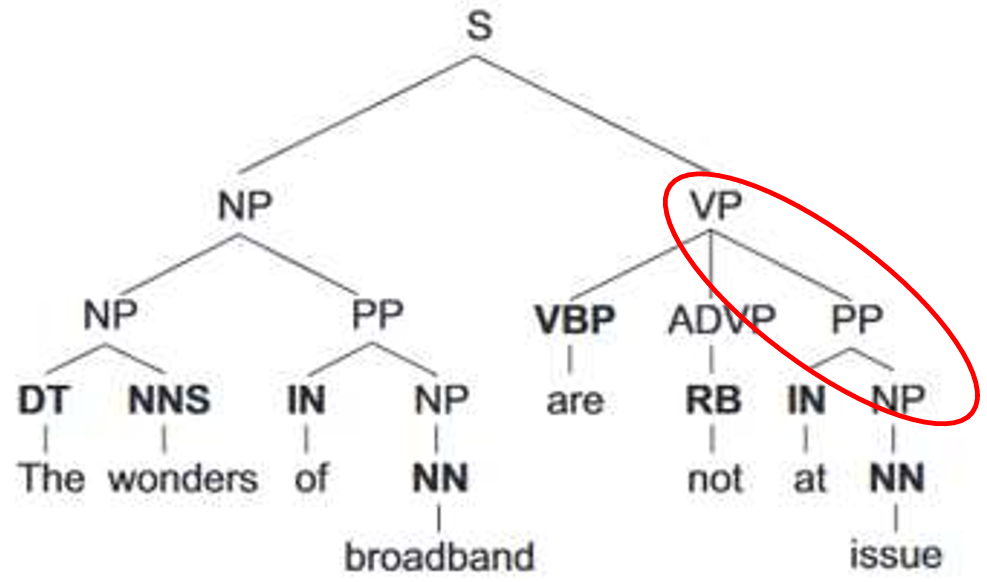
\includegraphics[width=.9\linewidth]{images/psg_2.png}
        \caption*{$2$\textsuperscript{nd}, $3$\textsuperscript{rd}, $4$\textsuperscript{th} order probabilities.}
    \end{subfigure}
    \begin{subfigure}{.32\textwidth}
        \centering
        \captionsetup{width=.8\linewidth}
        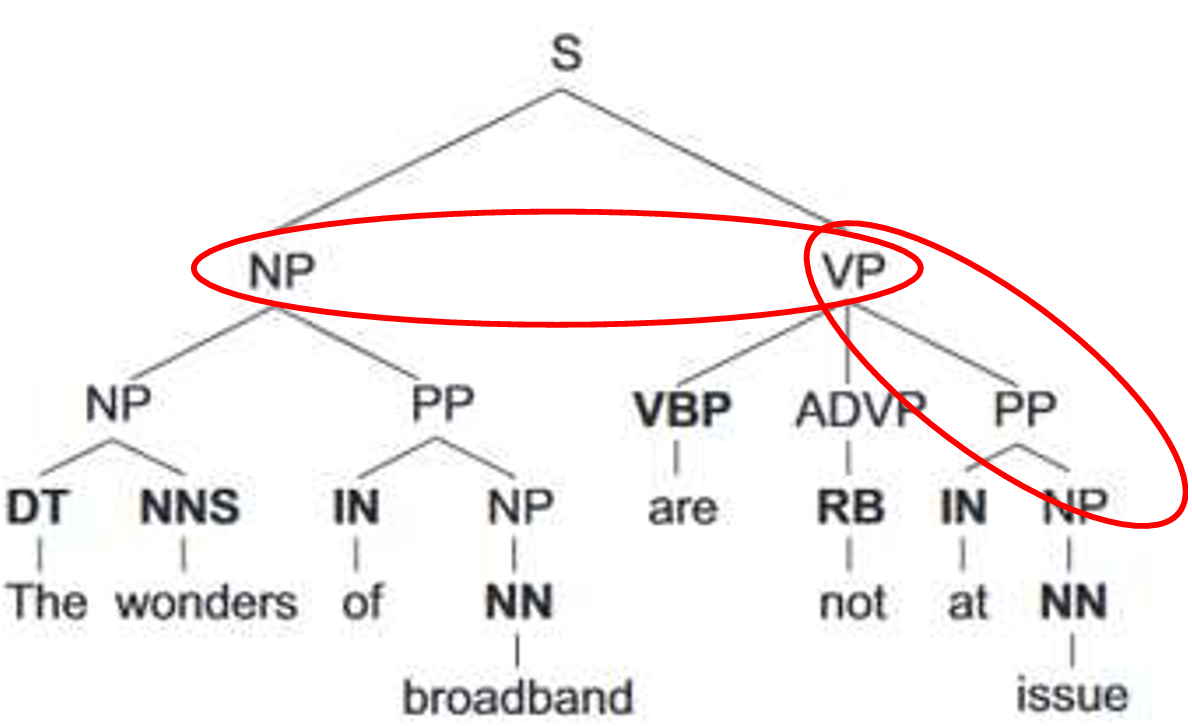
\includegraphics[width=.9\linewidth]{images/psg_3.png}
        \caption*{$2$\textsuperscript{nd}, $3$\textsuperscript{rd}, $4$\textsuperscript{th} order probabilities with left relation.}
    \end{subfigure}
    \caption{}
    \label{fig:psg_2}
\end{figure}

\subsection{Markov models}
They used Markov models of first, second, and third orders. In a Markov model of a given order ($n$), a symbol's probability dependds on the context of $n$ previous symbols only; that is, $P(w_t \vert w_{1\dots t-1})$ is taken to equal $P(w_t \vert w_{t-n\dots t-1})$. In their experiments, the probabilities of the sequences $w_{t-n\dots t-1}$ and $w_{t-n\dots t}$ are estimated from their occurrence frequencies in the training data. Note: a $4$\textsuperscript{th} order Markov model is quite good for the English language (it makes very good predictions).

\begin{figure}[!ht]
    \centering
    \captionsetup{width=.8\linewidth}
    \begin{subfigure}{.49\textwidth}
        \centering
        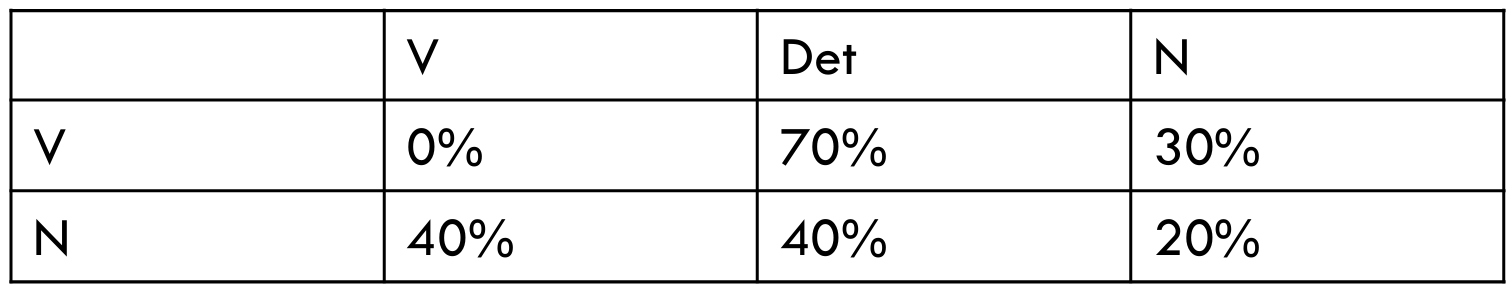
\includegraphics[width=.9\linewidth]{images/markov.png}
        \caption{First order Markov model.}
    \end{subfigure}
    \begin{subfigure}{.49\textwidth}
        \centering
        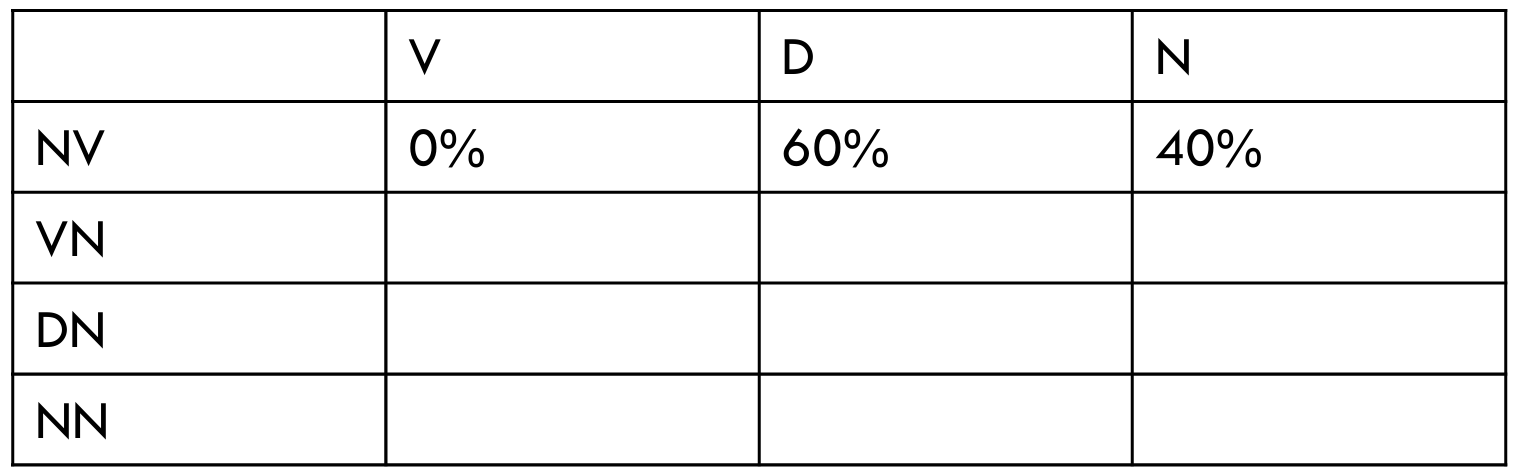
\includegraphics[width=.9\linewidth]{images/markov_2.png}
        \caption{$2$\textsuperscript{nd} order Markov model.}
    \end{subfigure}
    \caption{Examples of Markov models.}
    \label{fig:markov}
\end{figure}

\subsection{ESNs}
An ECN is a recurrent architecture that learns sequential relations between input elements without strict limitation on temporal integration window (long range relations as well)
It learns to predict a POS (the likelihood of the POS tag of the next word). Output activations are treated as probabilities over the upcoming POS tag, and the correct tag. The true POS of the next word is used as true target.

\subsection{Evaluation and results}
The basic idea for evaluating would be to look at how often the model makes a correct guess on the next word. However, it is difficult to do, so they look at how incorrect the model is. 
From each of the computational systems they derive a measure of Surprisal for the next word (POS). \textbf{All 3 approaches produce $p(w)$ in context}. 
They evaluate \textbf{Linguist Accuracy}: \textbf{how surprising is the POS for each system} (\textit{if the model is wrong, did it give high confidence?}). Presumably, the better a system learns stats of language, the less surprised it is by the future.
They also use a completely different statistics, \textbf{Psychological Accuracy}: how well do the surprise ratings produced by each model predict word reading time \notet.
The reading times are obtained with eye tracker for more than 2k sentences. This measure is quantified by variance reduced when Surprisal is added as explanatory variable to a baseline model including just word-frequency and word-length. Basically, they are asking whether it is the case that the model is surprised on the same words the people find difficult to read.

\osst{Reading time for people is a measure of surprise.}

The results (Fig. \ref{fig:frank_2}) show that, for very good linguistic accuracy, there are Markov processes that as good as PSG models (quite interesting).
RNNs (echo state networks) are the best in predicting human surprise, and in general the best psycho-linguistic models prove to be neural networks (rather than statistical models and grammars).

\begin{figure}[!ht]
    \centering
    \captionsetup{width=.8\linewidth}
    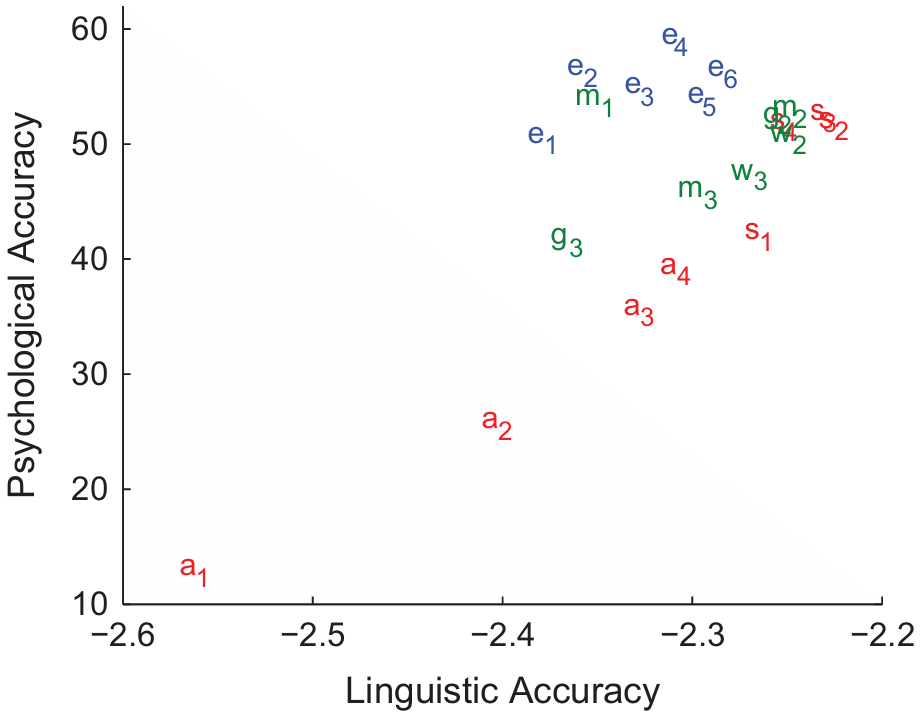
\includegraphics[width=0.4\linewidth]{images/frank_2.png}
    \caption{Results for first-pass reading times: psychological accuracy plotted against linguistic accuracy. Psychological accuracy was defined as the decrease in deviance that resulted from including one set of surprisal estimates in the regression, and linguistic accuracy was defined as the negative of the average surprisal. Results are plotted for phrase-structure-grammar (PSG) models, Markov models, and echo state networks. PSG models were constructed using only ancestor information (a$_n$, where $n$ indicates the number of levels up in the parse tree from which conditioning information was obtained) or taking also the ancestors' left siblings into account (s$_n$). Markov models of order $n$ were created with additive smoothing (m$_n$), Simple Good-Turing smoothing (g$_n$), or Witten-Bell smoothing (w$_n$). Echo state networks (e$_n$) had 100$n$ hidden units.}
    \label{fig:frank_2}
\end{figure}

